% 时间的变换与钟慢效应

\pentry{尺缩效应\upref{SRsmt}}




伽利略变换中时间是绝对而独立的,和空间无关.但我们在事件与尺缩效应\upref{SRsmt}词条中已经知道,引入光速不变原理之后会发现,两个独立事件\footnote{注意,我们已经声明过将同时同地的事件都看作同一个,因此此处的“独立事件”不可能是同时同地的.}是否同时,取决于观察的惯性系是哪个.

\subsection{测量事件发生时间}

在一个一维空间中,发生了一个事件,我们自然能知道这个事件发生的位置.实际上,因为我们要求事件发生的时候都同时发射一道球面光,在空间各个地方布满光感探测器以后,就可以通过探测的结果来反推球面光的形状,进而计算出球心位置.当然,我们没必要真的这么麻烦地计算,因为毕竟我们是在做思想实验,只需要明确“球面波的形状可测量”,进而得出“事件发生的位置是可知的”就行了.

但是事件发生的时间需要一点技巧去求得.很容易想到,利用光速不变原理就可以把对位置的知识转化成对时间的知识:首先让时间和空间的原点处($t=0, x=0$)发生一个事件,不妨称之为\textbf{参考事件}.在某时某地发生了另一个需要我们观测的事件,那么参考事件的球面光和待观测事件的球面光相遇也是一个事件.相遇事件发生的位置到原点的距离,除以光速,就可以得到相遇事件发生的时间;同理也可以得到相遇事件和待观测事件所发生的时间差,进而计算出待观测事件发生的时间.

\begin{figure}[ht]
\centering
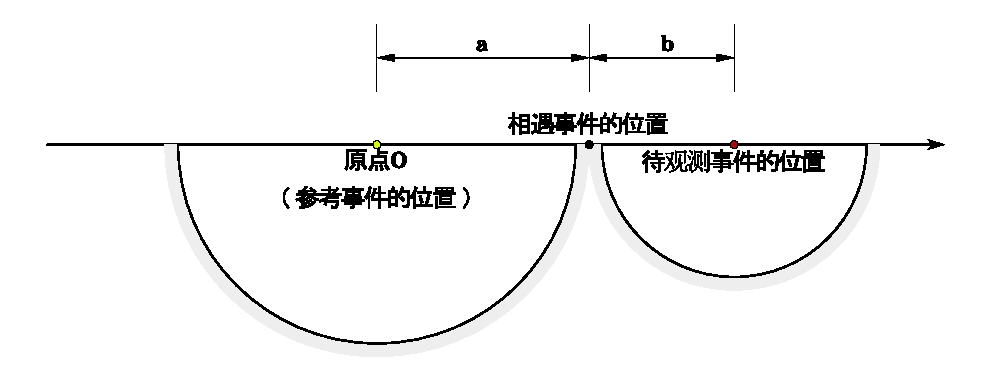
\includegraphics[width=14cm]{./figures/SRtime_1.pdf}
\caption{测量待观测事件发生的时间.相遇事件发生的时间是$a/c$,它和待观测事件的时间间隔是$-b/c$.也就是说,在如图所示的情形下,待观测事件发生的时间是$(a-b)/c=[2a-(a+b)]/c$.注意待观测事件的位置不是$b$,而是$a+b$.} \label{SRtime_fig1}
\end{figure}

这个方法在我们推导两个惯性系中时间的变换时非常好用.注意一点:我们要求相遇事件是参考事件的光球和待观测事件的光球\textbf{相切}的时候,不论是内切还是外切.外切可能出现在待观测事件是在负的时间上发生的的情况下——这时我们需要拓展事件光球的概念,在事件发生以前,光球向事件发生地收缩,在发生的那一刻收缩为点,重新发散出去.

\subsection{时间的变换}

沿用铁轨系$K_1$和火车系$K_2$的设定,令$K_2$相对$K_1$以速度$v$运动.我们现在想计算一下,在$K_1$中任意点$(x_1,t_1)$发生的事件,在$K_2$中应该对应哪个坐标$(x_2,t_2)$.由于这里的$x_1$是任意的,我们就需要火车无限长,不妨直接把火车和铁轨都抽象为一根无限长的坐标轴.

令两个坐标系的原点在各自的$t_1=0$,$t_2=0$时刻重合.我们可以任意指定一个事件,定义它在两个坐标系中的时空坐标都是$(0,0)$,从而实现“重合”的要求.这样一来,在两个坐标系的时空原点处发生的参考事件就成了同一个事件.

待观测事件在$K_1$中的坐标是$(x_1, t_1)$,意味着相遇事件在$K_1$中的坐标是$(t_1c+\frac{x_1-t_1c}{2}, t_1+\frac{x_1-t_1c}{2c})=(\frac{x_1+t_1c}{2},\frac{x_1+t_1c}{2c})$.注意相遇事件的时间和空间坐标中间只差了一个因子$c$,这是因为相遇事件必然在参考事件的光球上.由上一个小节知,利用相遇事件和待观测事件的空间坐标,就可以算出待观测事件的时间坐标;虽然我们已经知道了$t_1$,但你仍然可以验算一下,当作练习.

\begin{figure}[ht]
\centering
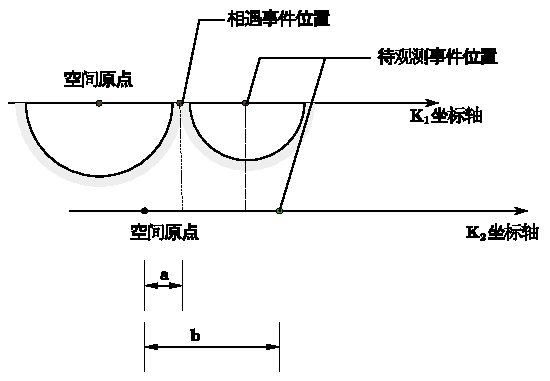
\includegraphics[width=12cm]{./figures/SRtime_2.pdf}
\caption{相遇事件在两个坐标轴中的表示.$a$是$K_2$中相遇事件的位置,$b$是$K_2$中待观测事件的位置.这个图是在$K_1$的视角下绘制的,请注意$K_2$坐标轴的尺缩效应使得$K_2$的尺子看起来更密集了一些.} \label{SRtime_fig2}
\end{figure}

同样地,我们知道相遇事件在$K_2$中待观测事件的位置是$(x_1-vt_1)/\sqrt{1-\frac{v^2}{c^2}}$\footnote{直接由尺缩效应得.$x_1-vt_1$部分是在$K_1$中看到的$K_2$的原点和待观测事件的距离.};类似地,相遇事件的位置\footnote{可以用$\frac{x_1+t_1c}{2}$代替$x_1$,$\frac{x_1+t_1c}{2c}$代替$t_1$,代入$(x_1-vt_1)/\sqrt{1-\frac{v^2}{c^2}}$得到.}  是$(\frac{x_1+t_1c}{2}-v\frac{x_1+t_1c}{2c})/\sqrt{1-\frac{v^2}{c^2}}=\frac{x_1+t_1c}{2}\cdot(1-\frac{v}{c})/\sqrt{1-\frac{v^2}{c^2}}$

代入\autoref{SRtime_fig1}的结果,可知$K_2$中待观测事件的时间是$[(x_1+t_1c)\cdot(1-\frac{v}{c})/\sqrt{1-\frac{v^2}{c^2}}-(x_1-vt_1)/\sqrt{1-\frac{v^2}{c^2}}]/c=\frac{t_1-\frac{v}{c}x_1}{\sqrt{1-\frac{v^2}{c^2}}}$.

由此,我们得出了时间的变换:$K_1$中的事件$(x_1, t_1)$,在$K_2$中的坐标是$((x_1-vt_1)/\sqrt{1-\frac{v^2}{c^2}}, (t_1-\frac{v}{c}x_1)/\sqrt{1-\frac{v^2}{c^2}})$.这就是\textbf{一维空间中的洛伦兹变换}.

\subsection{钟慢效应和孪生子悖论}

我们依然考虑火车系$K_2$和铁轨系$K_1$.在两个参考系的空间原点处放一只钟表,精确地记录着流逝的时间.火车上的钟表由于跟着火车一起运动,从\textbf{铁轨系}的视角来看,它的坐标随着时间$t_1$变化:$(vt_1, t_1)$.应用上一节的结论,可以计算出该钟表在\textbf{火车系}中的坐标:$(0, t_1\sqrt{1-\frac{v^2}{c^2}})$.空间坐标恒为零是肯定的,因为我们把它挂在了火车的原点上;时间坐标正比于$t_1$,但是乘以了一个小于$1$的因子$\sqrt{1-\frac{v^2}{c^2}}$.也就是说,在$K_1$看来,火车上的时间始终要过得比$K_1$中慢.

两个坐标系并没有哪个更特殊,所以可以简单地把钟慢效应理解为:以速度$v$运动的物体,其时间的流逝速度只有静止观察者手上那块表的时间流逝速度的$\sqrt{1-\frac{v^2}{c^2}}$.这里的时间流逝是最基本的物理性质,意味着如果一艘飞船相对你运动,在你看来飞船上的一切物理活动都变慢了,化学反应速率也以相同的比例变慢,质子衰变的速率也如此.

基于这个效应,人们自然提出了一个问题:如果有一对同年同月同日生的孪生子,一个人留在地球上,另一个人乘飞船高速远航.若干年后宇航孪生子回到地球,两人拥抱在一起.这时候,谁的年龄更大?

\textbf{孪生子悖论}困扰了学者们很长时间,直到广义相对论的提出才顺利解决.事实上,由于宇航员必须经历加速和减速过程,他相比地球上的孪生兄弟额外经历了引力场,引力场的钟慢效应弥补了这一“悖论”.结果是,宇航员会更年轻.至此,孪生子悖论已不再是悖论,所以通常也叫做\textbf{孪生子佯谬},佯谬意为“看起来是悖论但实际上不是”.

除此之外,还有根据尺缩效应构造的\textbf{潜艇佯谬}.假设有一艘潜艇悬浮在大海中,它的密度和水完全等同.现在潜艇水平向前运动,在大海看来,潜艇发生了尺缩,密度增加,应该开始下沉;但在潜艇看来是海水在运动,理应是海水密度增加,自己应该上浮.这个佯谬比起双生子佯谬要微妙得多,其解答也要涉及广义相对论理论.事实上,潜艇在这种情况下既上浮也下沉,因为有浮力的场合必有引力,潜艇的运动会导致它所看到的时空畸变,在潜艇看来自己在靠近海面,但是海底也会向上弯曲,接近潜艇.
